\documentclass[a4paper, 11pt]{beamer}

\mode<presentation>
{
  \usetheme{Madrid}
  % or ...
  %\usetheme{Darmstadt}
  \usefonttheme[onlylarge]{structurebold}
  \setbeamerfont*{frametitle}{size=\normalsize,series=\bfseries}
  \setbeamertemplate{navigation symbols}{}


  \setbeamercovered{transparent}
  % or whatever (possibly just delete it)
}

\usepackage{polski}
\usepackage[utf8]{inputenc}
\usepackage{times}
\usepackage[T1]{fontenc}
\usepackage{amsmath}

\title[info]
{
  Info krótkie
}

\author[Gal Anonim]
{
	Chack Norris ;-$)$
}

\institute[UwB]
{
  Uniwersytet w Białymstoku
}

\date[Białystok, 2012]
{
  Białystok, 2012
}

\begin{document}

  \begin{frame}{Legenda do obrazka}
    \begin{columns}
      \column{.6\textwidth}
	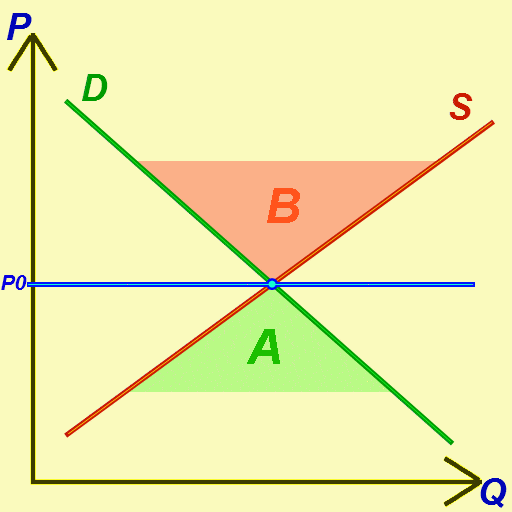
\includegraphics[width=7cm]{Price_of_market_balance.png}

      \column{.4\textwidth}
	Legenda:\\
	P – cena\\
	Q – ilość\\
	D – krzywa popytu\\
	S – krzywa podaży\\
	P0 – cena równowagi rynkowej\\
	A – nadwyżka popytu\\
	B – nadwyżka podaży\\
    \end{columns}
  \end{frame}

  \begin{frame}{Wzory matematyczne}{}
    {\color{blue}$f: \, A \hookrightarrow B$} -- zanurzenie zbioru $A$ w zbiór $B$. Zbiór $A$
    można wtedy utożsamić ze zbiorem $f(A) \subset B$,\\

    {\color{blue}int $A$} -- wnętrze zbioru $A$ (w przestrzeni, w której zbiór
    jest zanurzony),\\

    {\color{blue}$\arg \max_{x \in A} f(x)$} -- argument, przy którym funkcja
    $f$ osiąga wartość maksymalną na zbiorze $A$,\\

    {\color{blue}$<x, y> = \sum_{i=1}^n x_i y_i$} -- iloczyn skalarny wektorów
    $x, y \in \mathbb{R}^n$,\\

    {\color{blue}$\frac{df(x)}{dx}$} -- pochodna funkcji $f: \, R^1 \to R^1$ w
    punkcie $x$,\\

    {\color{blue}$\frac{df(x)}{dx}=\left( \frac{df_1(x)}{dx}, \cdots ,
    \frac{df_n(x)}{dx}\right )$} -- pochodna funkcji wektorowej $f=(f_1, \ldots
    , f_n)$,\\
    
    {\color{blue}$\frac{\partial f(x)}{\partial x}=\left( \frac{\partial f(x)}{\partial
    x_1}, \cdots , \frac{\partial f(x)}{\partial x_n} \right )$} -- gradient
    funkcji skalarnej,\\
    
    {\color{blue}$J(x) = \frac{\partial f}{\partial x} = \left( \frac{\partial
    f_i}{\partial x_j}\right)_{(n, n)}$} -- macierz funkcyjna
    Jacobiego.

  \end{frame}

  \begin{frame}{}
    $$x_1=\varphi_1(p, I)$$
    $$x_2=\varphi_2(p, I)$$
    $$x^0$$
    $$f(p)=\varphi(p, I(p))$$
    $$\{x \in \mathbb{R}_{+}^2 | <p, x> = I(p)\}$$
  \end{frame}

\end{document}
